\documentclass[12pt]{article}
\usepackage{amsmath}
\usepackage{amsthm}
\usepackage{amssymb}
\usepackage{euscript}
\usepackage{mathrsfs}
\usepackage{bm}
\usepackage{enumitem}
\usepackage{tikz}
\usepackage{mathtools}
\usepackage{float}
\usepackage{hyperref}
\usepackage{boldline}
\usepackage{indentfirst}
\usepackage{environ}
\usetikzlibrary{positioning}

\hypersetup{
    colorlinks=true,
    linkcolor=[RGB]{0,0,128},
    filecolor=magenta,
    urlcolor=cyan,
    citecolor = [RGB]{128,0,128}
}

\newcommand{\makeBox}[2] {
  \newsavebox{#1}
  \begin{lrbox}{#1}{#2}\end{lrbox}
}

\tikzstyle{tableau} = [y = -1cm, every node/.style={transform shape}]

\definecolor{gridColor}{RGB}{19,83,150}
\tikzstyle{dominoStyle} = [color=black, fill=white, rounded corners = .1cm, thick]
\tikzstyle{gridLine} = [color=gridColor, thick]
\tikzstyle{dominoText} = [font=\Large, midway]
\tikzstyle{cycleLine} = [color=green, thick, >->]
\tikzstyle{closedCycleLine} = [color=green, thick]
% \tikzstyle{fixedSquareStyle} = [pattern = crosshatch doats, pattern color=gridColor,  opacity=0.2]
\tikzstyle{fixedSquareStyle} = [color=gridColor,  opacity=0.07]
\tikzstyle{tileText} = [font=\large, midway]

\newcommand{\eps}{.06}
\newcommand{\teps}{\eps * 2}

% first entry is row, starting with 1, second entry is column, third is content
\newcommand{\filledSquare}[3]{\filldraw [dominoStyle] (#2 - 1 + \eps, #1 - 1 + \eps) rectangle + (1 - \teps, 1 -\teps) node [tileText] {$#3$};}
% The fourth entry shifts vertically
\newcommand{\filledSquareShift}[4]{\filldraw [dominoStyle] (#2 - 1 + #4 + \eps, #1 - 1 + \eps) rectangle + (1 - \teps, 1 -\teps) node [tileText] {$#3$};}

\newcommand{\horizontalDomino}[3]{\filldraw [dominoStyle] (#2 - 1 + \eps, #1 - 1 + \eps) rectangle + (2 - \teps, 1 -\teps) node [dominoText] {$#3$};}
\newcommand{\verticalDomino}[3]{\filldraw [dominoStyle] (#2 - 1 + \eps,  #1 - 1 + \eps) rectangle + (1 - \teps,2 -\teps) node [dominoText] {$#3$};}

\newcommand{\horizontalDominoShift}[4]{\filldraw [dominoStyle] (#2 - 1 + #4 + \eps, #1 - 1 + \eps) rectangle + (2 - \teps, 1 -\teps) node [dominoText] {$#3$};}
\newcommand{\verticalDominoShift}[4]{\filldraw [dominoStyle] (#2 - 1 + #4 + \eps,  #1 - 1 + \eps) rectangle + (1 - \teps,2 -\teps) node [dominoText] {$#3$};}

\newcommand{\zeroSquare}[2]{\filldraw [dominoStyle] (#2 - 1 + \eps, #1 - 1 + \eps) rectangle + (1 - \teps, 1 -\teps) node [dominoText] {$0$};}
\newcommand{\zeroSquareShift}[3]{\filldraw [dominoStyle] (#2 - 1 + #3 + \eps, #1 - 1 + \eps) rectangle + (1 - \teps, 1 -\teps) node [dominoText] {$0$};}


\newcommand{\emptyBox}[2]{\filldraw [dominoStyle] (#2 - 1 + \eps, #1 - 1 + \eps) rectangle + (2 - \teps, 2 -\teps);}
\newcommand{\signedBox}[3]{
\filldraw [opacity=0] (#2 - 1 + 1, #1 - 1) rectangle + (1, 2) node [dominoText,opacity=1] {$#3$};
\filldraw [dominoStyle, fill opacity = 0] (#2 - 1 + \eps, #1 - 1 + \eps) rectangle + (2 - \teps, 2 -\teps);
}

\newcommand{\emptyBoxShift}[3]{\filldraw [dominoStyle] (#2 - 1 + #3 + \eps, #1 - 1 + \eps) rectangle + (2 - \teps, 2 -\teps);}
\newcommand{\signedBoxShift}[4]{
\filldraw [opacity=0] (#2 - 1 + 1 + #4, #1 - 1) rectangle + (1, 2) node [dominoText,opacity=1] {$#3$};
\filldraw [dominoStyle, fill opacity = 0] (#2 - 1 + #4 + \eps, #1 - 1 + \eps) rectangle + (2 - \teps, 2 -\teps);
}

% These rows and columns are zero-based
\newcommand{\horizontalGridLine}[3]{\draw [gridLine] (#1, #2) -- + (#3,0);}
\newcommand{\verticalGridLine}[2]{\draw [gridLine] (#1, 0) -- + (0,#2);}
\newcommand{\fixedSquare}[2]{\filldraw [fixedSquareStyle] (#1,#2) rectangle +(1,1);}

% This will have #1 * 2 rows and #2 *2 columns
\newcommand{\gridLines}[2] {
  \pgfmathsetmacro{\verticalEnd}{2 * #1}
  \pgfmathsetmacro{\horizontalEnd}{2 * #2}
  \foreach \vertical in {0,...,#2} {
    \pgfmathsetmacro{\var} {2 * \vertical}
    \verticalGridLine{\var}{\verticalEnd}
  }
  \foreach \horizontal in {0,...,#1} {
    \pgfmathsetmacro{\var} {2 * \horizontal}
    \horizontalGridLine{0}{\var}{\horizontalEnd}
  }
}

% This will have #1 * 2 rows and #2 *2 columns
% The vertical lines will be shifted over #3 squares
\newcommand{\gridLinesShift}[3] {
  \pgfmathsetmacro{\verticalEnd}{2 * #1}
  \pgfmathsetmacro{\horizontalEnd}{2 * #2}
  \foreach \vertical in {0,...,#2} {
    \pgfmathsetmacro{\var} {2 * \vertical + #3}
    \verticalGridLine{\var}{\verticalEnd}
  }
  \foreach \horizontal in {0,...,#1} {
    \pgfmathsetmacro{\var} {2 * \horizontal}
    \horizontalGridLine{#3}{\var}{\horizontalEnd}
  }
}

\newcommand{\fixedSquaresStart}[4]{
  \foreach \row in {#1,...,#2} {
    \foreach \column in {#3,...,#4} {
      \pgfmathsetmacro{\var}{\row + \column}
      \ifodd \var
      \else
        \fixedSquare\column\row
      \fi
    }
  }
}

\newcommand{\fixedSquares}[2]{
  \foreach \row in {0,...,#1} {
    \foreach \column in {0,...,#2} {
      \pgfmathsetmacro{\var}{\row + \column}
      \ifodd \var
        \fixedSquare\column\row
      \fi
    }
  }
}

% This has #1 * 2 rows and #2 * 2 columns
\newcommand{\fixedSquaresForGrid}[2] {
  \pgfmathsetmacro{\rowParameter}{#1 * 2 - 1}
  \pgfmathsetmacro{\columnParameter}{#2 * 2 - 1}
  \fixedSquares{\rowParameter}{\columnParameter}
}

% This has #1 * 2 rows and #2 * 2 columns
% The vertical lines will be shifted over #3 squares
\newcommand{\fixedSquaresForGridShift}[3] {
  \pgfmathsetmacro{\rowParameter}{#1 * 2 - 1}
  \pgfmathsetmacro{\columnStart}{#3}
  \pgfmathsetmacro{\columnEnd}{#2 * 2 - 1 + #3}
  \fixedSquaresStart{0}{\rowParameter}{\columnStart}{\columnEnd}
}

\newcommand{\fixedSquaresStartAlt}[4]{
  \foreach \row in {#1,...,#2} {
    \foreach \column in {#3,...,#4} {
      \pgfmathsetmacro{\var}{\row + \column + 1}
      \ifodd \var
      \else
        \fixedSquare\column\row
      \fi
    }
  }
}

% This has #1 * 2 rows and #2 * 2 columns
% The vertical lines will be shifted over #3 squares
\newcommand{\fixedSquaresForGridShiftAlt}[3] {
  \pgfmathsetmacro{\rowParameter}{#1 * 2 - 1}
  \pgfmathsetmacro{\columnStart}{#3}
  \pgfmathsetmacro{\columnEnd}{#2 * 2 - 1 + #3}
  \fixedSquaresStartAlt{0}{\rowParameter}{\columnStart}{\columnEnd}
}


% This will have #1 rows and #2 columns
\newcommand{\typeAGridLines}[2] {
  \foreach \vertical in {0,...,#2} {
    \verticalGridLine{\vertical}{#1}
  }
  \foreach \horizontal in {0,...,#1} {
    \horizontalGridLine{0}{\horizontal}{#2}
  }
}

% This will have #1 rows and #2 columns
% The vertical lines will be shifted over #3 squares
\newcommand{\typeAGridLinesShift}[3] {
  \foreach \vertical in {0,...,#2} {
    \pgfmathsetmacro{\var} {\vertical + #3}
    \verticalGridLine{\var}{#1}
  }
  \foreach \horizontal in {0,...,#1} {
    \horizontalGridLine{#3}{\horizontal}{#2}
  }
}

\newcommand{\sij}{{S_{ij}}}
\renewcommand{\ss}[2]{{S_{#1,#2}}}

\begin{document}
  The next property of the sign tableaux is that dominoes in a type II cycle are paired with dominoes in the type I cycle which they are immediately nested in.
  Specifically, each domino in a type II cycle with fixed square $\sij$ is paired with the domino with fixed square $\ss{i-1}{j-1}$.
  Paired dominoes either both have no sign or else they have opposite signs.
  In the following example, I'm showing the two sign tableaux out of the four tableaux.
  Blue diagonal lines indicate the pairing of fixed squares.

  \begin{figure}[H]
    \centering
    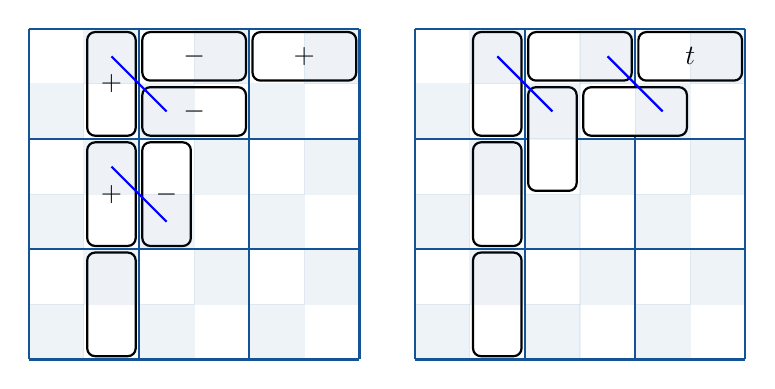
\begin{tikzpicture}[tableau, scale = .7]
      \gridLines{3}{3}
      \verticalDomino{1}{2}{+}
      \verticalDomino{3}{2}{+}
      \horizontalDomino{1}{3}{-}
      \horizontalDomino{2}{3}{-}
      \horizontalDomino{1}{5}{+}
      \verticalDomino{3}{3}{-}
      \verticalDomino{5}{2}{}
      \fixedSquaresForGrid{3}{3}

      \draw[thick, blue] (1.5, .5) -- +(1, 1);
      \draw[thick, blue] (1.5, 2.5) -- +(1, 1);

      \gridLinesShift{3}{3}{7}
      \verticalDominoShift{1}{2}{}{7}
      \verticalDominoShift{3}{2}{}{7}
      \horizontalDominoShift{1}{3}{}{7}
      \verticalDominoShift{2}{3}{}{7}
      \horizontalDominoShift{1}{5}{t}{7}
      \horizontalDominoShift{2}{4}{}{7}
      \verticalDominoShift{5}{2}{}{7}
      \fixedSquaresForGridShift{3}{3}{7}

      \draw[thick, blue] (1.5 + 7, .5) -- +(1, 1);
      \draw[thick, blue] (3.5 + 7, .5) -- +(1, 1);
    \end{tikzpicture}
  \end{figure}


  One way to think about the paired dominoes is in analogy with the $Sp(p,q)$ algorithm.
  In the $Sp(p,q)$ algorithm, the signs at the end of even rows were important for the algorithm, and had to do with cycles, but they had no information about the nilpotent orbit.
  After the algorithm was done, they were forgotten.
  In the same way, in the $SO(p,q)$ algorithm, paired dominoes have no information about the union of nilpotent orbits which is the associated variety.
  After the algorithm is done, the paired dominoes are boxed up and forgotten.
  In particular, though associated varieties are constant on cells, the sign tableaux of the algorithm are not.
  For example, a parameter which produces the two signed tableaux shown above is in the same cell as parameters which produce the folllowing pair of signed tableaux, which are more easily seen as representing unions of nilpotent orbits:
  \begin{figure}[H]
    \centering
    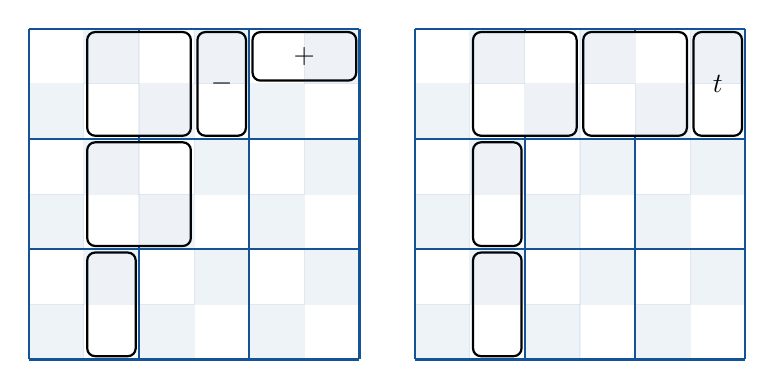
\begin{tikzpicture}[tableau, scale = .7]
      \gridLines{3}{3}
      \emptyBox{1}{2}
      \emptyBox{3}{2}
      \verticalDomino{1}{4}{-}
      \horizontalDomino{1}{5}{+}
      \verticalDomino{5}{2}{}
      \fixedSquaresForGrid{3}{3}

      \gridLinesShift{3}{3}{7}
      \emptyBoxShift{1}{2}{7}
      \emptyBoxShift{1}{4}{7}
      \verticalDominoShift{3}{2}{}{7}
      \verticalDominoShift{1}{6}{t}{7}
      \verticalDominoShift{5}{2}{}{7}
      \fixedSquaresForGridShift{3}{3}{7}
    \end{tikzpicture}
  \end{figure}

  Before describing more rules for the sign tableaux, I'll explain how they correspond to unions of nilpotent orbits.
  This will put the next rules in a context.
  To be specific, I'll talk about the left sign tableau, where the signs are $+$ and $-$.
  From the point of view of a nilpotent orbit, a domino with a $+$ sign is holding two $+$ signs.
  A blank domino is holding one $+$ sign and one $-$ sign.
  A 2x2 box is holding two $+$ signs and two $-$ signs.

  For example, from the discrete series parameter $1{+}\ 2-$, we get the following four tableaux:
  \begin{figure}[H]
    \centering
    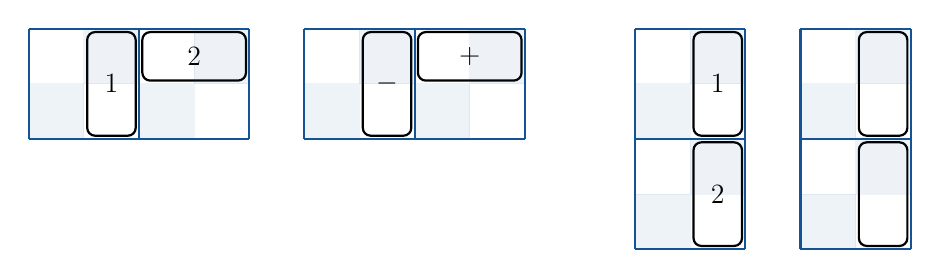
\begin{tikzpicture}[tableau, scale = .7]
      \gridLines{1}{2}
      \verticalDomino{1}{2}{1}
      \horizontalDomino{1}{3}{2}
      \fixedSquaresForGrid{1}{2}

      \gridLinesShift{1}{2}{5}
      \verticalDominoShift{1}{2}{-}{5}
      \horizontalDominoShift{1}{3}{+}{5}
      \fixedSquaresForGridShift{1}{2}{5}

      \gridLinesShift{2}{1}{11}
      \verticalDominoShift{1}{2}{1}{11}
      \verticalDominoShift{3}{2}{2}{11}
      \fixedSquaresForGridShift{2}{1}{11}

      \gridLinesShift{2}{1}{14}
      \verticalDominoShift{1}{2}{}{14}
      \verticalDominoShift{3}{2}{}{14}
      \fixedSquaresForGridShiftAlt{2}{1}{14}
    \end{tikzpicture}
  \end{figure}

  The first sign tableau has two $+$ signs and one $-$ sign in its first row, and one $-$ sign in its second row.
  So, it denotes the nilpotent orbit
  \begin{figure}[H]
    \centering
    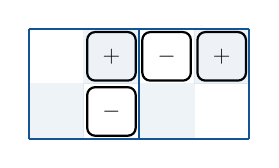
\begin{tikzpicture}[tableau, scale = .7]
      \gridLines{1}{2}
      \filledSquare{1}{2}{+}
      \filledSquare{1}{3}{-}
      \filledSquare{1}{4}{+}
      \filledSquare{2}{2}{-}
      \fixedSquaresForGrid{1}{2}
    \end{tikzpicture}
  \end{figure}

  On the other hand, if we start with the parameter $1s\ 2s$, which is discrete series for the dual group, we get
  \begin{figure}[H]
    \centering
    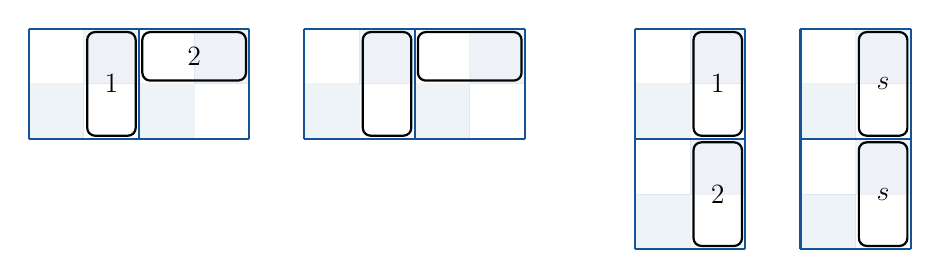
\begin{tikzpicture}[tableau, scale = .7]
      \gridLines{1}{2}
      \verticalDomino{1}{2}{1}
      \horizontalDomino{1}{3}{2}
      \fixedSquaresForGrid{1}{2}

      \gridLinesShift{1}{2}{5}
      \verticalDominoShift{1}{2}{}{5}
      \horizontalDominoShift{1}{3}{}{5}
      \fixedSquaresForGridShift{1}{2}{5}

      \gridLinesShift{2}{1}{11}
      \verticalDominoShift{1}{2}{1}{11}
      \verticalDominoShift{3}{2}{2}{11}
      \fixedSquaresForGridShift{2}{1}{11}

      \gridLinesShift{2}{1}{14}
      \verticalDominoShift{1}{2}{s}{14}
      \verticalDominoShift{3}{2}{s}{14}
      \fixedSquaresForGridShiftAlt{2}{1}{14}
    \end{tikzpicture}
  \end{figure}
  Now, the first sign tableau, with its blank dominoes, signifies the union of the two nilpotent orbits shown below.
  \begin{figure}[H]
    \centering
    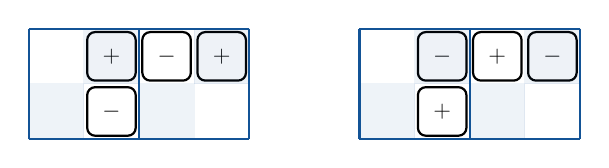
\begin{tikzpicture}[tableau, scale = .7]
      \gridLines{1}{2}
      \filledSquare{1}{2}{+}
      \filledSquare{1}{3}{-}
      \filledSquare{1}{4}{+}
      \filledSquare{2}{2}{-}
      \fixedSquaresForGrid{1}{2}

      \gridLinesShift{1}{2}{6}
      \filledSquareShift{1}{2}{-}{6}
      \filledSquareShift{1}{3}{+}{6}
      \filledSquareShift{1}{4}{-}{6}
      \filledSquareShift{2}{2}{+}{6}
      \fixedSquaresForGridShiftAlt{1}{2}{6}
    \end{tikzpicture}
  \end{figure}

  This is because the blank vertical domino contains two signs, one $+$ sign and one $-$ sign, and it is not specified which one is in the first row and which is in the second row.

  This introduces the next rule of sign tableaux.
  Unlike in previous algorithms, here you don't have unpaired dominoes with different signs in the same column.
  Instead, a column can have unpaired dominoes with one given sign and also blank dominoes.
  Similarly, in a row, the unpaired dominoes alternate in sign, but they can be separated by one or more blank dominoes.

  The equivalence relation is that you can interchange adjacent unpaired dominoes if one has a sign and one is blank, as long as you also interchange the corresponding dominoes in the other sign tableau, and as long as both tableaux then still obey all the rules of sign tableaux.
  One difference from previous algorithms is that each equivalence class has a preferred representative, namely that in which signed dominoes are as far up and to the right as possible.
  At the end of each stage of the algorithm, the tableaux need to end up in the preferred representative.
  However, as you perform a step of the algorithm, you might need to interchange some dominoes.

  There are complicated rules for what configurations are possible for the paired dominoes, and how they interact with adjacent unpaired dominoes when interchanges are made.
\end{document}
